\section{Background} 
In recent years, Personal Informatics or Quantified Self (QS) tools have received an increasing interest in the field of human-computer interaction with the introduction of low-cost mobile applications, wearables and advances in sensor technologies. Personal Informatics help people understand themselves through self-tracking of \textit{"personally relevant information for the purpose of self-reflection and gaining self-knowledge"} \cite{Li2010}. 

\subsection{Stages of Self-Tracking}
Researchers have proposed different models for understanding, how self-trackers concretely use Personal Informatics tools over time. Li et al. proposed the cascading five-staged \textit{Personal Informatics Model} describing, how self-trackers transition between: (1) \textit{Preparation} (determining variables, tools and frequency of tracking), (2) \textit{collection} (logging data), (3) \textit{integration} (preparing data for reflection e.g. by aggregating and analysing data), (4) \textit{reflection} (examining data to gain self-knowledge) and (5) \textit{action} (deciding what to do with said knowledge) \cite{Li2010}. 

Comparing Personal Informatics and telehealth literature, we found differences in roles of stakeholders illustrated on Figure \ref{fig:StakeholdersModel}. In telehealth, healthcare providers mandate and predefine what symptoms, how often and with what tool patients should track (\textit{preparation}). Patients collect both objective numerical (e.g. oxygen saturation measures) and subjective binary data (e.g. yes/no answers to whether dyspnea has increased more than usual) (\textit{collection}). The system integrates the data and based on predefined individual “normal ranges” flags data for follow-ups (\textit{integration}). Trained nurses or physicians review the self-tracked data (\textit{reflection}) in telehealth and if needed contact and advise the patient on potential initiation of treatment (\textit{action}) \cite{piloting, pedone}. 

\begin{figure}[!h]
\centering
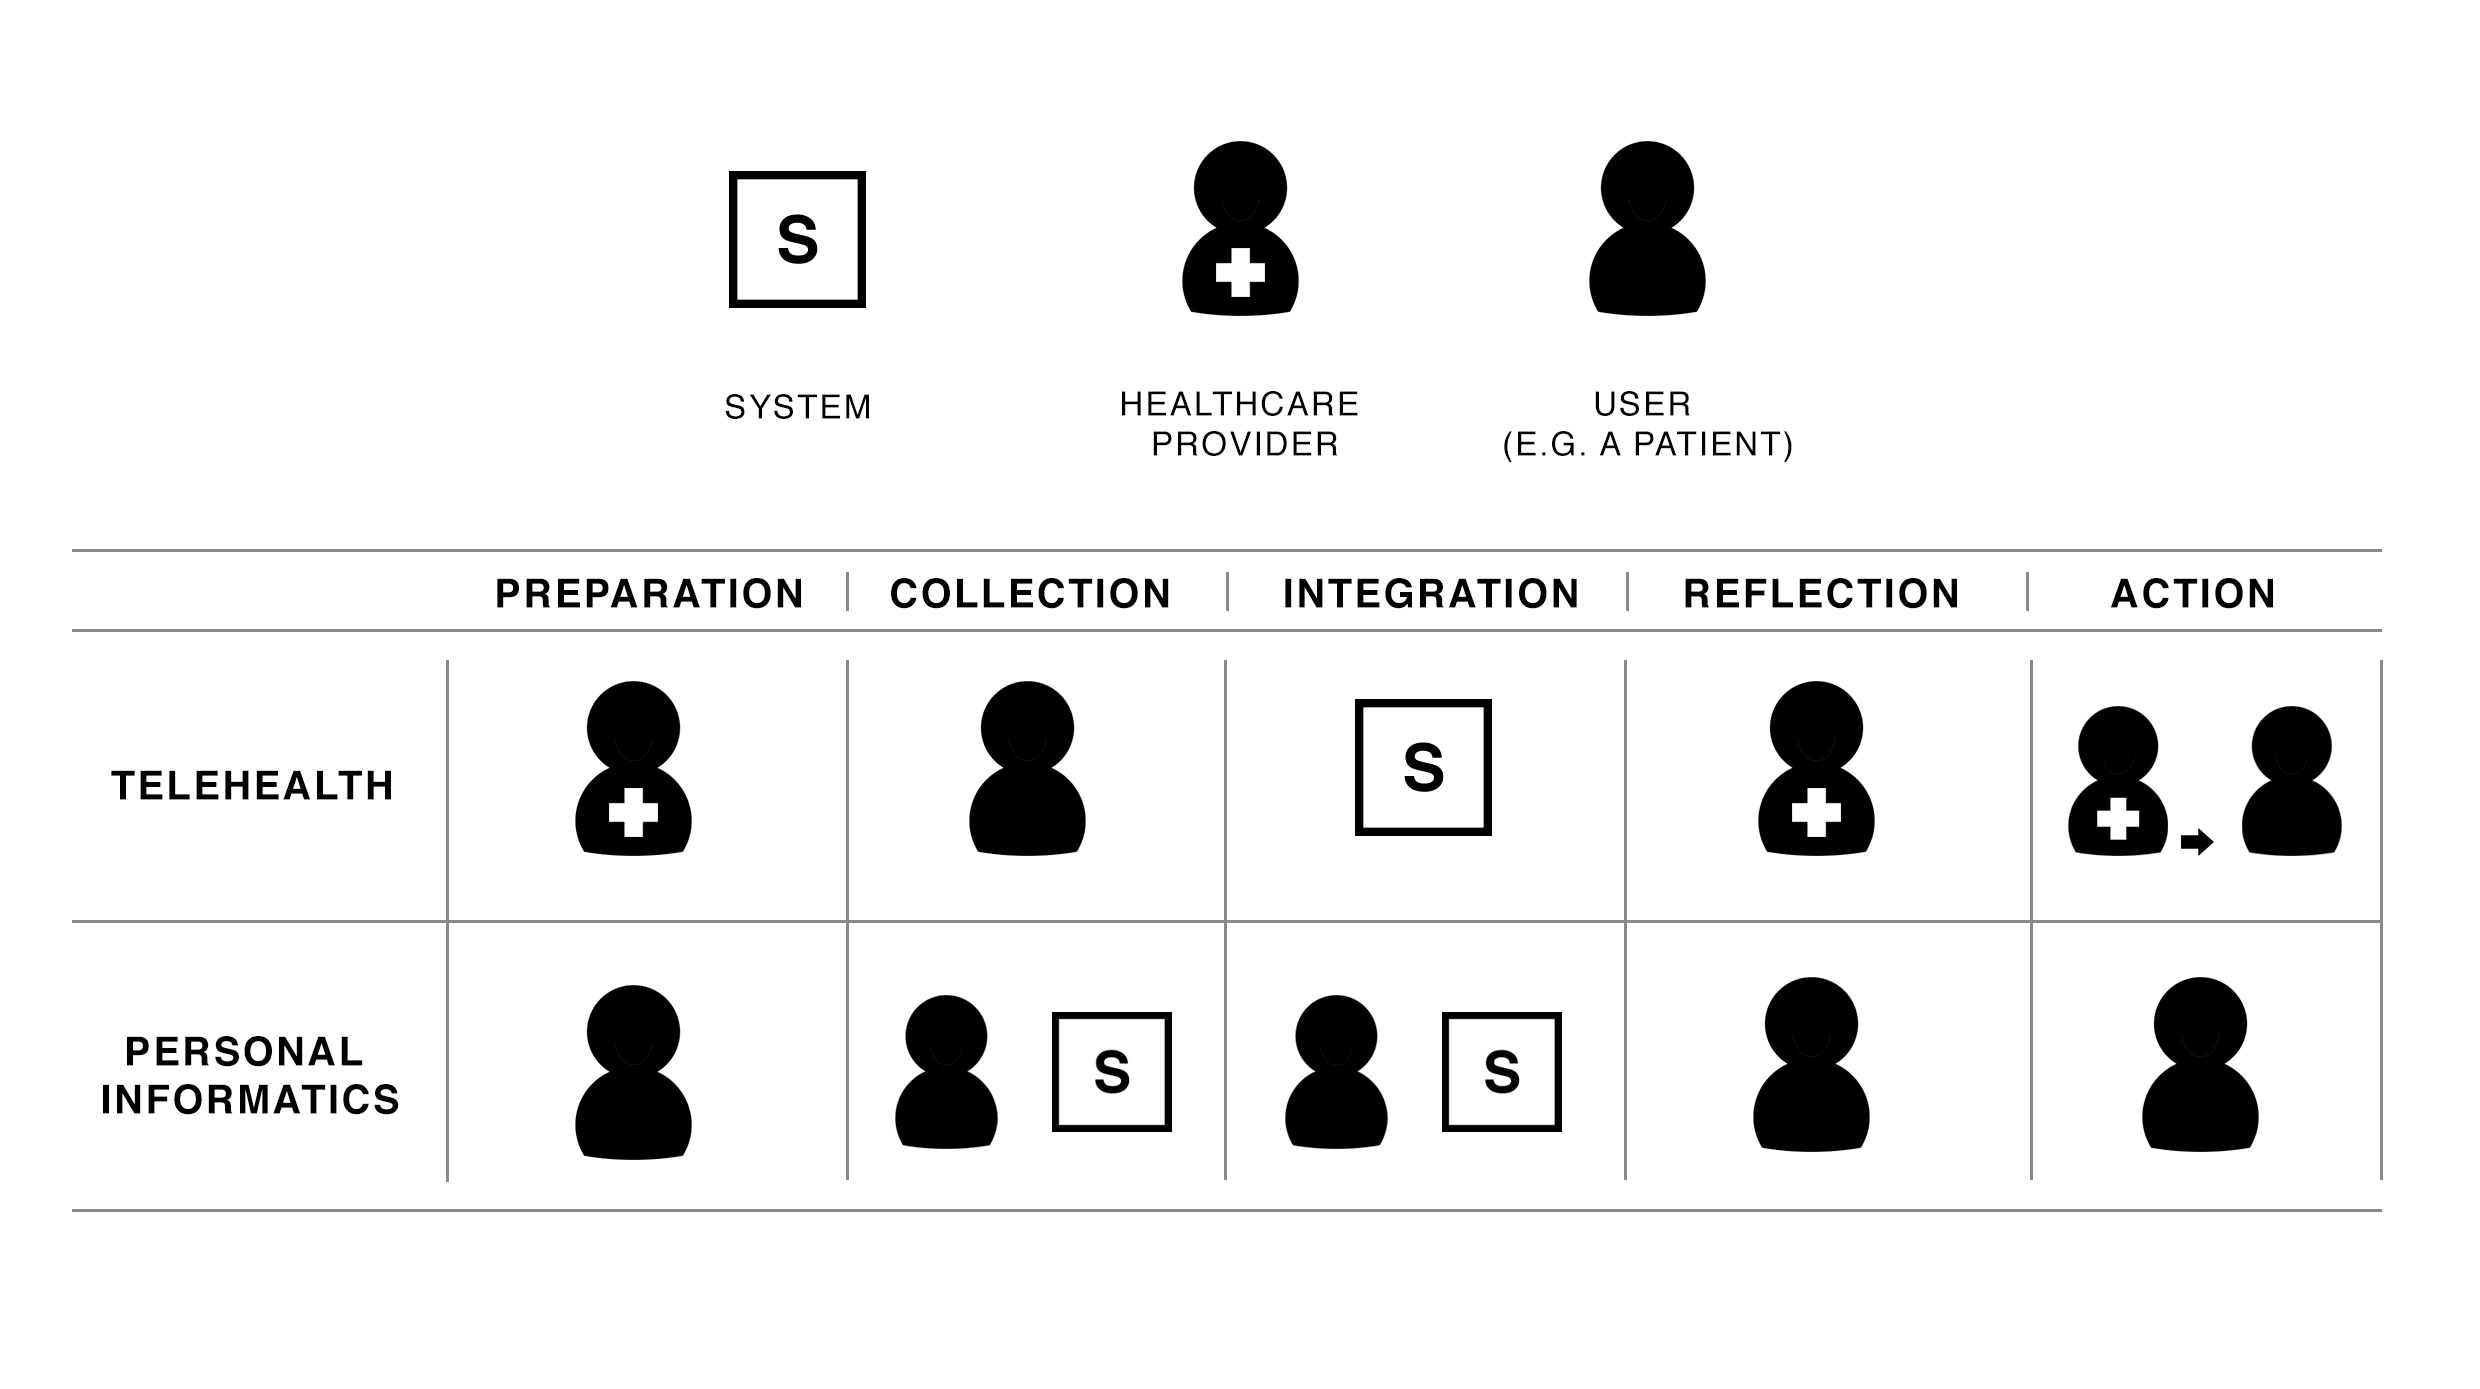
\includegraphics[width=0.9\columnwidth]{img/StakeholdersModel}
\caption{Roles of in Personal Informatics and telehealth}
\label{fig:StakeholdersModel}
\end{figure}

Epstein et al. showed that \textit{collection}, \textit{integration} and \textit{reflection} are ongoing processes that can occur simultaneously and categorized these activities as \textit{tracking and acting}. They further divided the \textit{preparation} stage into \textit{deciding} (to self-track) and \textit{selecting} (a tool to track with) and integrated \textit{lapsing} (e.g. due to an oversight or holidays) and \textit{resuming} into their \textit{Lived Informatics Model} \cite{Epstein2015, Rooksby2014}. 

Rivera-Pelayo et al. discussed Personal Informatics in light of reflective learning theory (or learning by reflection) \cite{Rivera}. Based on the work of Boud et al., they proposed a framework consisting of three dimensions in which technology can be integrated to support reflection: (1) \textit{Tracking}, (2) \textit{triggering} and (3) \textit{recalling and revisiting}. \textit{Tracking} consist of logging data that serves as the basis for the reflective process. Data can both be experiences (e.g. feelings or physiological data), but also outcomes (e.g. gained insight or changes in behaviour). \textit{Triggers} have the purpose of raising awareness and detect discrepancies. These are related to the initiation of reflection based on the logged data. Finally, enrichment (i.e. enriching the tracked data with e.g. context data) and data presentation (i.e. visualising the data) have the purpose of facilitating \textit{recall and revisit} of past experiences. 

We use the \textit{Lived Informatics Model} \cite{Epstein2015} and Rivera-Pelayo’s framework as an analytical lens to identify user needs and barriers for self-tracking and synthesize findings from literature. We aim to provide an understanding of, how technology has and can be used to support people in their self-tracking efforts in the following section. 

\subsection{Preparation} 
The \textit{preparation} stage includes people getting motivated to track (e.g. because of a goal they have in mind), which guides the decision on, what data to track and selecting the tool to track with. 

\subsubsection{Motivation and Goals} 
Epstein et al., found that people self-tracked for various reasons, but not all people self-tracked with a concrete goal in mind \cite{Epstein2015}. One example is people, who tracked out of natural curiosity about what their data might reveal about themselves \cite{Li2010, Epstein2015}. We refer to this as self-tracking for \textit{life experience}. From the literature, we classified four main drivers for sustained tracking among people with a health-related condition: (1) \textit{documentation} (e.g. to create records for their healthcare providers \cite{Ancker2015}), (2) \textit{communication} (e.g. to communicate their condition to family members \cite{MacLeod2014}), (3) \textit{self-knowledge and advice} (e.g. to get a sense of the current state of their condition or to get advice from their healthcare-provider \cite{MacLeod2014, Ancker2015}) and (4) \textit{self-improvement} (e.g. to change or maintain a behaviour in order to improve well-being or lifestyle \cite{MacLeod2014, Ancker2015, Chung2016}).

Barriers to motivation included strong emotional adversity to reflection on data, because it reminded people of negative aspects of their illness \cite{Li2010, Ancker2015}, tracking the wrong data or not tracking well enough to gain benefits \cite{Chung2015}, effort \cite{Choe2014, Patel2012}, reliability and relevance \cite{Oh2015, piloting, Epstein2015} and mismatches between subjective feeling and objective measures \cite{Ancker2015}. 

\subsubsection{Selection of Data and Tool} 
Patel et al. found that, sometimes healthcare providers gave little support on what symptoms to track and how to track (e.g. frequency of tracking) \cite{Patel2012}. This is an issue in health conditions that involve many symptoms that arise unexpectedly, where patients have to decide on additional symptom tracking \cite{Patel2012, Chung2016}. Trackers used tools, such as notebooks, health diaries and specific applications to do additional tracking or sometimes developed tools themselves that were cumbersome and incomplete \cite{Patel2012}. This later affected the \textit{integration} and \textit{reflection} stages, where healthcare providers struggled with interpreting data sets with additional and not always relevant information \cite{Chung2015, Chung2016}.

Little is known about what motivates to self-track in telehealth. As previously mentioned (See Figure \ref{fig:StakeholdersModel}), the decision on what data to track and which tool to use, is in telehealth context decided by a healthcare provider. This potentially has an effect on the acceptance from the user and the efficiency of learning by reflection, as mentioned by Rivera et al. \cite{Rivera}.

\subsection{Collection} 
The \textit{collection} stage deals with logging data. Self-tracker find logging too many things challenging and leading to tracking fatigue \cite{Choe2014, Patel2012}. Logging, however, is a prerequisite for triggering and supporting \textit{reflection}. It is thus of importance to choose as unobtrusive a method as possible that is sufficiently reliable \cite{Muller}. We previously described self-tracking as logging data (either objective or subjective) during concrete \textit{episodes} over time. We now distinguish between data being either \textit{automatically} logged (e.g. physiological sensors that log heart rate) and \textit{manually} logged (e.g. self-reporting feelings or self-measured value). 

\subsubsection{Manual Logging}
Manual logging requires responsibility and motivation that has to be kept over time from trackers and can therefore be burdensome compared to automatic logging \cite{Li2010, Muller}. Some self-trackers found manual logging time consuming and requiring effort \cite{Ancker2015}, hampering incorporation of tracking into daily routines \cite{Verdezoto2015, Ancker2015}. E.g. when objective data had to be manually logged, it required preparation time, e.g., resting before taking physiological measures, which increased time and effort \cite{Verdezoto2015}. Data granularity impeded logging, because  trackers had to overthink in order to rate mood on a scale from 0 to 10 \cite{Oh2015} and lack of baseline to compare with caused difficulties for trackers with chronic conditions, when self-reporting on severity of symptoms, because they were constantly symptomatic \cite{piloting}. Another downside of manual logging is that self-trackers sometimes postpone manual logging \cite{MacLeod2014}, which induces recall bias that affects data reliability. 

\subsubsection{Automatic Logging}
Automatic logging shifts the effort from the trackers to the technology. It allows for configuration of frequency and precision, but also implies challenges in terms of filtering and aggregating the large amounts \cite{Muller}. One of the main downsides of automatic logging is that it might reduce awareness and self-reflection \cite{Choe2014, Li2011}.

\subsection{Integration}
The \textit{integration} stage can be more or less apparent to the tracker depending on whether integration is automatically done by the system, requiring less effort from the self-tracker \cite{Li2010}. Previous studies show that self-trackers sometimes postponed data exploration, when integration did not happen automatically, since it involved tedious tasks, such as cleaning up data, formatting and running statistical tests \cite{Choe2014, Chung2015, Li2010}. 

Systems that require manual integration expect the user to be able to analyse the data and ascertain the best way of creating a representation. Whooley et al. found that this is of interest to curiosity-driven self-trackers that want to integrate data manually and explore the novel insights that data can offer them. In contrast, self-trackers with a goal, knew what they were looking for in the data and strived at using automatic integration systems, allowing them to concentrate on reflection. The manual integration process is an iterative process of moving back and forth between representation creation and reflection \cite{Whooley2014}. 

\subsection{Reflection}
In the \textit{reflection} stage, self-trackers reflect on the collected and integrated data by looking, exploring or interacting with visualisations of it \cite{Li2010}. While literature points at many different definitions of reflection, we found little about how reflection can be evaluated. Fleck \& Fitzpatrick identified five different ‘levels of reflection’ (R0-R4) that indicate what types of activities and behaviours can be associated with reflection \cite{Fleck}. Levels consist of (R0) describing or stating without being reflective (\textit{description}), (R1) describing with explanations in a reportive or descriptive way (\textit{reflective description}), (R2) seeing things from different perspectives and trying to identify relationships (\textit{dialogic reflection}), (R3) changing original point of view due to gained knowledge (\textit{transformative reflection}) and (R4) seeing the wider perspective beyond the immediate context (\textit{critical reflection}). While higher level indicates being more reflective, lower levels are prerequisites for becoming more reflective. 

\subsubsection{Conditions for Reflection}
One of the condition for reflection is creating and allowing for time to reflect, according to Fleck \& Fitzpatrick \cite{Fleck}. Li et al. distinguished between short-term reflection, where the self-tracker reflects immediately after logging the data and long-term reflection that might occur several days or weeks after \cite{Li2010}. While short-term reflection makes the tracker aware of the current status, long-term reflection allows for higher levels of reflection (at least R2), since the tracker can compare logged data between different times and explore trends and patterns. 

Several authors mention that the one reflecting should be open-minded and willing to reflect \cite{Atkins, Rogers}. As mentioned by Atkins et al., in some literature there is an implicit assumption that \textit{skills} (such as critical analysis and evaluation) are necessary to engage in reflection \cite{Atkins, Rogers}. Fleck \& Fitzpatrick mention that reflection skills can be developed with time and with the right support \cite{Fleck}.

The reflective process needs a trigger. People often need a reason (e.g. a purpose) or at least an encouragement to reflect \cite{Fleck, Mols}. In psychology, Festinger’s cognitive dissonance theory describes, how a mismatch (psychological discomfort or dissonance) between an individual's attitude and behaviour can lead to rethinking one’s attitude and behaviour \cite{Rivera}. 

Rivera et al. mention that dissonance triggers reflection and can be actively triggered (system explicitly tries to catch the user’s attention by highlighting a certain mismatch) or passively triggered (system only presenting the data and relying on the user to detect something that starts a reflective process). Dissonance may occur due to comparison between current level and a recommended level or goal, but some might prefer such comparison in response to oneself. For example, Ancker et al. found that some self-trackers prefered to interpret their data in light of their own personal and medical history and/or symptoms, rather than striving for provider-recommended “normal ranges” \cite{Ancker2015}. In the following we describe different ways to trigger and support reflection identified in our literature review. 

\subsubsection{Reflective Questions or Prompting}
One way of supporting reflection is through the use of reflective questions or prompts. Simply asking people to provide justification or explanation for e.g. events or actions can support \textit{reflective description} (R1) \cite{Fleck}. The presence of another person can encourage reflection, especially in a dialogue among two “uneven partners” (i.e. two people not sharing the same understanding or experience), where one takes the role of asking questions. 

Systems can also take this leading role of asking questions, but opposed to the previously mentioned example, where reflection among two people can be “dialogue driven”, systems often only pose an initial reflective question \cite{Mols}. An intelligent system could further support reflection through follow-up questions. Another ways to foster reflection is by prompting questions triggered by automatically logged context data \cite{Fleck}. Presenting data that is not usually visible encourages people to see things from another perspective and can potentially lead to looking for relationships and patterns (R2) according to Fleck \& Fitzpatrick. 

\subsubsection{Visualisations}
Despite simply looking at data is not considered reflective according to Fleck \& Fitzpatricks’ levels of reflection, creating representation of data is considered a prerequisite to support higher reflective levels \cite{Fleck}. Visualisations of data can help people in exploring their information and gaining insights \cite{Li2010, Choe2014}. 

When designing visualisations, it is important to consider under which conditions reflection is to take place (e.g. time and effort expected from the user, skills and purpose for reflection) \cite{Cuttone, Muller}. Li et al. identified six types of questions people ask about their self-tracked data \cite{Li2011}. These are, getting to know (1) status (what is current status?), (2) history (what has status been in the past?), (3) goals (what goal is appropriate to pursue?), (4) discrepancies (how does current status compare to goal?), (5) context (what affects current status?), (6) factors (how are different variables related?). Depending on the conditions, supporting both simple (e.g. status charts) and detailed visualisations (e.g. of time series) can be important \cite{Muller, Cuttone}.

Often people want to obtain answers to their question (e.g. status) without spending too much time or effort, which can be done on a simplified dashboard representation that allows for a quick overview \cite{Cuttone}. M{\"u}ller et al. found that people used status charts to quickly get an overview of their data and used it as a starting point for exploration \cite{Muller}. Comparison charts were requested in their study to benchmark against other people in the sense-making process and to assess success. However, as previously mentioned, some prefer that such benchmarking occurs in response to oneself \cite{Ancker2015}. 

Previous literature shows that visualisation of time series data can support revisiting and analysing past experiences (history) and trigger storytelling about experiences behind data \cite{Rivera, Muller}. It can foster reflection on global trends e.g. on upward and downward trends or deviations from a historical normal (suggesting a problem) \cite{Rivera}. Cuttone et al. mentioned that human behaviour is often characterized by periodic patterns, but that time series graphs do not facilitate exploring such patterns \cite{Cuttone}. They instead proposed using calendar heatmap representations using different color shades to indicate variable values. Visualisations of multiple time series can support reflection on how multiple variables are related or how multiple variables change over time \cite{Cuttone}. 

Visualisations of time series can further be combined with discrete events \cite{Sorensen} to support reflective description (R1). Previous studies showed barriers for reflection involved that tools did not always support either simple visualisations of data or more complex features (e.g. filtering data to focus on a subset of data, zooming out to get an overview or comparing multiple variables) \cite{Li2011, MacLeod2014}. 

\subsubsection{External activities}
While reflection is an internal process, it can occur when trying to externalize thoughts and feelings e.g. in diaries or during reflective writing \cite{Mols}. These activities are often descriptive or emotional (R1). Recording reflection outcomes for later revisiting and reflection on gained insights has been proposed as another way to support reflection \cite{Isaac, Muller}. Isaac et al. found that allowing for writing down thoughts helped people explore and understand their feelings \cite{Isaac}. 

\subsection{Action} 
People decide what \textit{action} to take based on the findings from the \textit{reflection} stage. Epstein et al. found that trackers who had other motivations than behaviour change, e.g. self-understanding, did not reach this stage \cite{Epstein2015}. Trackers who tracked for self-improvement sometimes lacked the knowledge necessary to identify the appropriate actions to take, such that they could regulate their progress towards their behaviour change goal. This happened either because they collected irrelevant data \cite{Choe2014, Chung2015} (e.g. food and symptoms, instead of ingredients that triggered the symptoms) or because they needed actionable (expert) advice \cite{Verdezoto2015, Li2010, Oh2015}. Several studies found that most Personal Informatics systems do not provide actionable advice \cite{Chung2015, Li2010, Verdezoto2015}.

\section{Research area}
In summary, previous literature shows user needs and concerns during tracking activities, but little is known about these aspects, when tracking is monitored by a healthcare provider as in telehealth. It is unclear how concrete design decisions regarding entry and interaction with data affect reflection. In the following studies, we explore user needs and concerns when self-tracking in telehealth and how we can design to support users' self-tracking needs. 
